% ${framed}

\documentclass[9pt,addpoints]{exam}
\usepackage{dsfont}
\usepackage{amsfonts}
\usepackage{amsmath}
\usepackage{array}
\usepackage{tabularx}
\usepackage{etoolbox}
\usepackage{eso-pic}
\usepackage{hyperref}
\usepackage{color}

\usepackage[letterpaper,top=1.55cm, bottom=3.5cm, outer=4cm, inner=3cm,
            heightrounded, marginparwidth=0cm,marginparsep=1cm]{geometry}

\newtoggle{compress}
\toggletrue{compress}
%\togglefalse{compress}

\hypersetup{
  pdftitle={Test 1 for Math 1113, Fall 2018},
  pdfsubject={Precalculus},
  pdfauthor={Kelly Black},
  pdfkeywords={graph-transformations, domain, range, distance, lines, quadratics},
  anchorcolor = {red},
  colorlinks = {true},
  %% pdfpagemode={FullScreen}
}
 

\usepackage{tikz}
\usepackage{pgf}
\usepackage{pgfplots}
\usepgfplotslibrary{fillbetween}
%%\pgfplotsset{width=7cm}
\usepgfplotslibrary{patchplots}


%%\oddsidemargin=-0.5in
%%\evensidemargin=-0.5in
%%\textwidth=6.5in

%%\topmargin=-0.75in
%%\textheight=9.5in

\pagestyle{plain}
 \reversemarginpar

\pointpoints{pt}{pts}
\bracketedpoints

\def\Course{Math 1113}
\def\Instructor{Andrew Maurer}
\def\NumSec{}
%% \def\time{12:00pm-12:50pm}
\def\Date{Fall 2018}
\def\test{Test 1}
\def\version{A}


 \pagestyle{headandfoot}
 \headrule
 \firstpageheader{\bf 
   UGA Dept of Mathematics \\ % 
   \Course}
 {\large \textbf{\test} }
 {\Instructor \\ \Date}
  \runningheadrule
  \runningheader{\Course}
               {\test %%, Section \NumSec
               }
               {\Date}
 \footrule
 \firstpagefooter{\version}
                 {Page \thepage\ of \numpages}
                 {}
 \runningfooter  {\version}
                 {Page \thepage\ of \numpages}
                 {\rule{0cm}{.35cm} Points earned: \hbox to
                 1cm{\hrulefill} \\  %
                  out of a possible \pointsonpage{\thepage} points}
%%%%%%%%%%%%%%%%%%%%%%%%%%%%%%%%%%%%%%%%%%%%%%%%%%%%%%%%%%%%%%%%%%%
 \extrawidth     { 1.00in}
  \extraheadheight{0.15in}%[-0.30in]{-0.30in}
 \extrafootheight{-0.41in}
 \addpoints
 %%%%%%%%%%%%%%%%%%%%%%%%%%%%%%%%%%%%%%%%%%%%%%%%%%%%%%%%%%%%%%%%%%%

\newcommand{\pointBox}{\marginpar[\begin{minipage}{1cm}\hfill\vspace*{1cm}
    ~ \\ \rule{1.5cm}{0.2mm}\end{minipage}]{~}}


\newcommand{\laplace}[1]{\makebox{$ {\cal L} \{ #1 \}$}}
\newcommand{\vi}{\makebox{$\vec{\imath}$}}
\newcommand{\vj}{\makebox{$\vec{\jmath}$}}
\newcommand{\vk}{\makebox{$\vec{k}$}}
\newcommand{\lp}{\left(}
\newcommand{\rp}{\right)}
%%\newcommand{\half}{\frac{1}{2}}




\begin{document}


%% <%include file="coverPage.template"/>

\noindent
\begin{tabular}{ll@{\hspace{3em}}ll@{\hspace{3em}}ll}
  %%%%\multicolumn{4}{l}{\textit{You must acknowledge that this is your
  %%%%work by signing:} } \\ %

  \multicolumn{4}{m{\textwidth}}{
  By providing my signature below  I acknowledge
  that I  abide by the University's academic honesty policy.
  This is my work, and I did not get any help from anyone else
  during the exam:} \\ [25pt] \\
  
  Name (sign):    & \rule{5cm}{0.2mm} & 
                                        Name (print):   & \rule{5cm}{0.2mm}  \\ [20pt]
  Student Number: & \rule{5cm}{0.2mm} \\ [20pt]
  Instructor's Name: & \rule{5cm}{0.2mm} & Class Time: & \rule{4cm}{0.2mm}
\end{tabular}


%%\bonustotalformat{Common Knowledge}

\vqword{
  \begin{minipage}[h]{5em}
    ~ \\Problem \\ Number \\ [-8pt]
  \end{minipage}
}
\vpword{
  \begin{minipage}[h]{5em}
    ~ \\ Points \\ Possible \\ [-8pt]
  \end{minipage}
}
%%\cvbpword{
%%  \begin{minipage}[h]{5em}
%%    ~ \\ Bonus \\ Points \\ [-8pt]
%%  \end{minipage}
%%}
\vsword{  \begin{minipage}[h]{5em}
    ~ \\ Points \\ Made \\ [-8pt]
  \end{minipage}
}

\newenvironment{nagging}%
  {\begin{itemize}%
    \setlength{\itemsep}{6pt}%
    \setlength{\parskip}{0pt}}%
  {\end{itemize}}

\vfill

\begin{tabular}{p{8cm}m{8cm}}
  \gradetable[v][questions]
  %%\partialgradetable{main}[v][questions]
  %%\partialbonusgradetable{bonus}
  %%\combinedgradetable[v][questions]
  &
    \begin{nagging}
    \item If you need extra space use the last page.

    \item Please show your work. \textbf{An unjustified answer may receive
        little or no credit.}

    \item If you make use of a theorem to justify a conclusion then
      state the theorem used by name.

    \item Your work must be {\bf neat}. If I can't read it (or can't
      find it), I can't grade it.

    \item The total number of possible points that is assigned for
      each problem is shown here.  The number of points for each
      subproblem is shown within the exam.

    \item Please turn off your mobile phone.

    %\item You are only allowed to use a TI-30 calculator. No other
    %  calculators are permitted.

    \item A calculator is not necessary, but numerical answers should
      be given in a form that can be directly entered into a
      calculator.



    \end{nagging}
\end{tabular}

\vfill



\bonuspointpoints{Point Common Knowledge}{Bonus}


\clearpage 

%% <%include file="defaults.template"/>
%% <%include file="overallreport.template"/>

\bonuspointpoints{Point Common Knowledge}{Points Bonus}

\clearpage


\begin{questions}
 \question Use the function below to answer questions 1(a), 1(b), and 1(c).  Keep your numeric values exact.\[f(x) = \dfrac{\sqrt{x} - 5}{x^2-9}\]

  \begin{parts}
    \part[5] \pointBox ~ Determine the \textbf{$x$-intercept(s)} of $f(x)$.

    %% <%include file="questionResults.template"/>    

    \iftoggle{compress}{\vfill}{~\\}

    \part[5] \pointBox ~ Determine the \textbf{domain} of $f(x)$.  Give your answer in interval notaton.

    %% <%include file="questionResults.template"/>    

    \iftoggle{compress}{\vfill}{~\\}

    \part[5] \pointBox ~ The function $g(x)$ is created by moving $f(x)$ one unit to the left.  Determine the formula for $g(x)$.  You do not have to simplify your function.

    %% <%include file="questionResults.template"/>    

    \iftoggle{compress}{\vfill}{~\\}

  \end{parts}


  \iftoggle{compress}{\clearpage}

 \question Use the function below to answer questions 2(a), 2(b), and 2(c).  Keep your numeric values exact.\[f(x) = 4x^2 - 12x + 5\]

  \begin{parts}
    \part[5] \pointBox ~ Determine the \textbf{$x$-intercept(s)} of $f(x)$.

    %% <%include file="questionResults.template"/>    

    \iftoggle{compress}{\vfill}{~\\}

    \part[5] \pointBox ~ Determine the \textbf{$y$-intercept(s)} of $f(x)$.

    %% <%include file="questionResults.template"/>    

    \iftoggle{compress}{\vfill}{~\\}

    \part[5] \pointBox ~ Determine the \textbf{range} of $f(x)$.  Give your answer in interval notaton.

    %% <%include file="questionResults.template"/>    

    \iftoggle{compress}{\vfill}{~\\}

  \end{parts}


  \iftoggle{compress}{\clearpage}
  
   \question A point $P$ has coordinates $(3, -5)$.  Answer the following.

  \begin{parts}
    \part[5] \pointBox ~ Let point $Q$ be at the origin.  Determine the length of the line segment $\overline{PQ}$.

    %% <%include file="questionResults.template"/>    

    \iftoggle{compress}{\vfill}{~\\}

    \part[5] \pointBox ~ Determine an equation for the line \textbf{perpendicular} to $4x + 3y = 7$ that contains the point $P$.

    %% <%include file="questionResults.template"/>    

    \iftoggle{compress}{\vfill}{~\\}

    \part[5] \pointBox ~ Determine an equation for the \textbf{vertical line} containing the point $P$.

    %% <%include file="questionResults.template"/>    

    \iftoggle{compress}{\vfill}{~\\}

  \end{parts}


  \iftoggle{compress}{\clearpage}
  

   \question Let $f(x)$ = $3x - 2$ and $g(x) = 17 - x^2$.  Answer the following:

  \begin{parts}
    \part[5] \pointBox ~ Compute $(f - g)(x)$.  Simplify your answer completely.

    %% <%include file="questionResults.template"/>    

    \iftoggle{compress}{\vfill}{~\\}

    \part[5] \pointBox ~ Compute $(f \circ g)(x)$.  Simplify your answer completely.

    %% <%include file="questionResults.template"/>    

    \iftoggle{compress}{\vfill}{~\\}

    \part[5] \pointBox ~ Compute $(g \circ f)(x)$.  Simplify your answer completely.

    %% <%include file="questionResults.template"/>    

    \iftoggle{compress}{\vfill}{~\\}

  \end{parts}


  \iftoggle{compress}{\clearpage}
  
  
  \question A business has a monthly fixed cost of \$3500, which includes rent, utilities, and labor.  They have a variable cost of \$1.55 per item that they produce.  Define $x$ as the number of items that they produce on a monthly basis.  Use this information to answer the following:
  
  
  \begin{parts}
  \part[5] \pointBox Denote $C$ as their total \textbf{monthly cost} (measured in dollars) of operations.  Determine the formula for $C(x)$.

    \iftoggle{compress}{\vspace{14em}}{~\\} 

  \part[10] \pointBox The company will break even when they sell exactly 2500 items.  Determine what price they will need to set in order to make this happen.

    \iftoggle{compress}{\vfill}{~\\} 

    %% <%include file="questionResults.template"/>        



  \end{parts}

    \iftoggle{compress}{\clearpage}{} 



  \question Answer each of the questions below, and the function
    referred to is defined by
    \begin{eqnarray*}
      f(x) & = & \left\{
                              \begin{array}{c@{\hspace{3em}}rcl}
                                -3x - 4 & x & < & 2 \\ \\
                                (x+2)^3 - 4 & x & \geq & 2
                              \end{array}
                              \right.
    \end{eqnarray*}


  \begin{parts}
  \part[3] Determine the value for $f(-2)$.
      \iftoggle{compress}{\vspace{14em}}{~\\} 
  \part[3] Determine the value for $f(3)$.
      \iftoggle{compress}{\vspace{14em}}{~\\} 
      
  \part[4]   Determine the average rate of change of the function from
      $x=-2$ to $x=3$.

      \iftoggle{compress}{\vspace{30em}}{~\\}             


    %% <%include file="questionResults.template"/>


  \end{parts}


  \iftoggle{compress}{\clearpage}


\question \pointBox A rectangular field will be fenced on all four sides. There will also be two lines of fence across the field, parallel to the shorter side, which has length $x$ ft.  (See diagram below.). Answer the following.

\[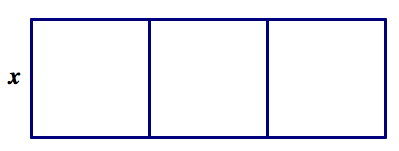
\includegraphics[width=3.5in]{t1.png}\]
  \begin{parts}
   \part[6] If 4400 ft of fencing are available to create the field, determine a function $A(x)$ that models the area of the rectangular field. (Notice that $A(x)$ is a function only of $x$.)


    \iftoggle{compress}{\vspace{14em}}{~\\} 



  \part[9] Determine the dimensions of the field will
produce the maximum area.

    %% <%include file="questionResults.template"/>

    \iftoggle{compress}{\vfill}{~\\} 

    

  \end{parts}


  
  \iftoggle{compress}{\clearpage}
    

\end{questions}



Extra space for work. \textbf{Do not detach this page.} If you want us to consider the work on this
    page you should print your name, instructor and class meeting time below. \\ [10pt]
    Name (print): \rule{3cm}{0.2mm} Instructor (print):
    \rule{3cm}{0.2mm}  Time: \rule{3cm}{0.2mm}


    \iftoggle{compress}{\vfill}{~\\}



\end{document}


